\section{Characterising Pressure Source}\label{sec:static_test}
\subsection{Initial Test}
The first step in characterising the system was to investigate the static pressure losses present in the tank without a piston or any powder. This immediately presented a problem as the static pressure readings were far below expected, as seen in figure \autoref{fig:static-pressure-drop-3bar}. 
\begin{figure}[htbp]
    \centering

    \begin{minipage}{0.45\textwidth}
        \centering
        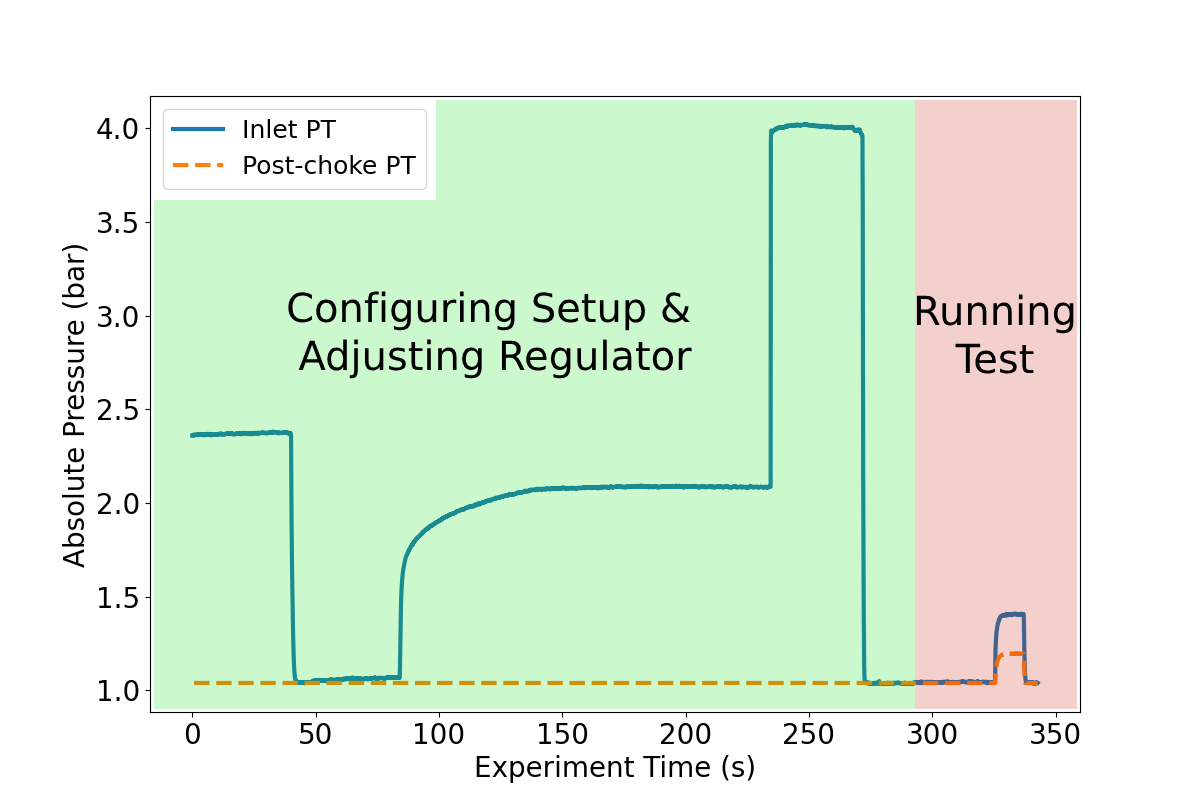
\includegraphics[width=\textwidth]{../report_assets/3_bar_static_full.png}
        \caption{Full 4 bar test.}\label{fig:static-pressure-drop-3bar_full}
    \end{minipage}
    \hfill
    \begin{minipage}{0.45\textwidth}
        \centering
        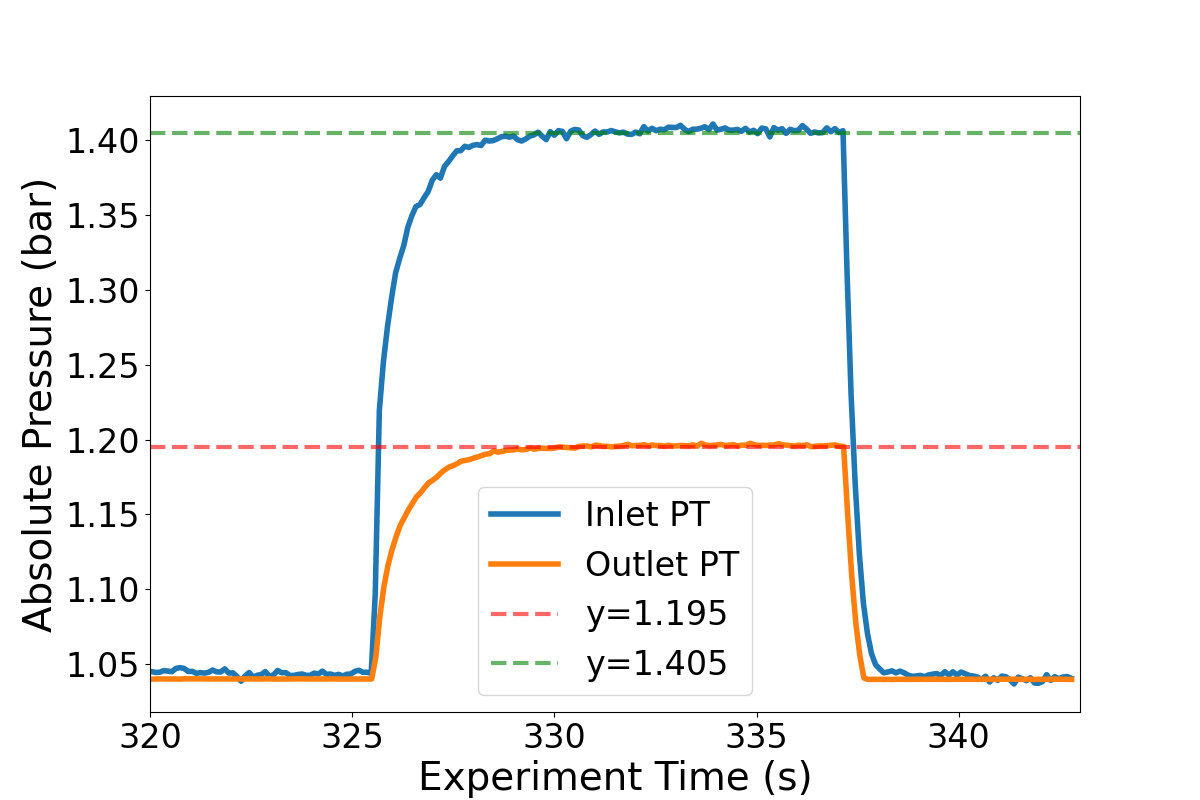
\includegraphics[width=\textwidth]{../report_assets/3_bar_static.png}
        \caption{Static pressure from 4 bar.}\label{fig:static-pressure-drop-3bar}
    \end{minipage}
    \begin{minipage}{0.45\textwidth}
        \centering
        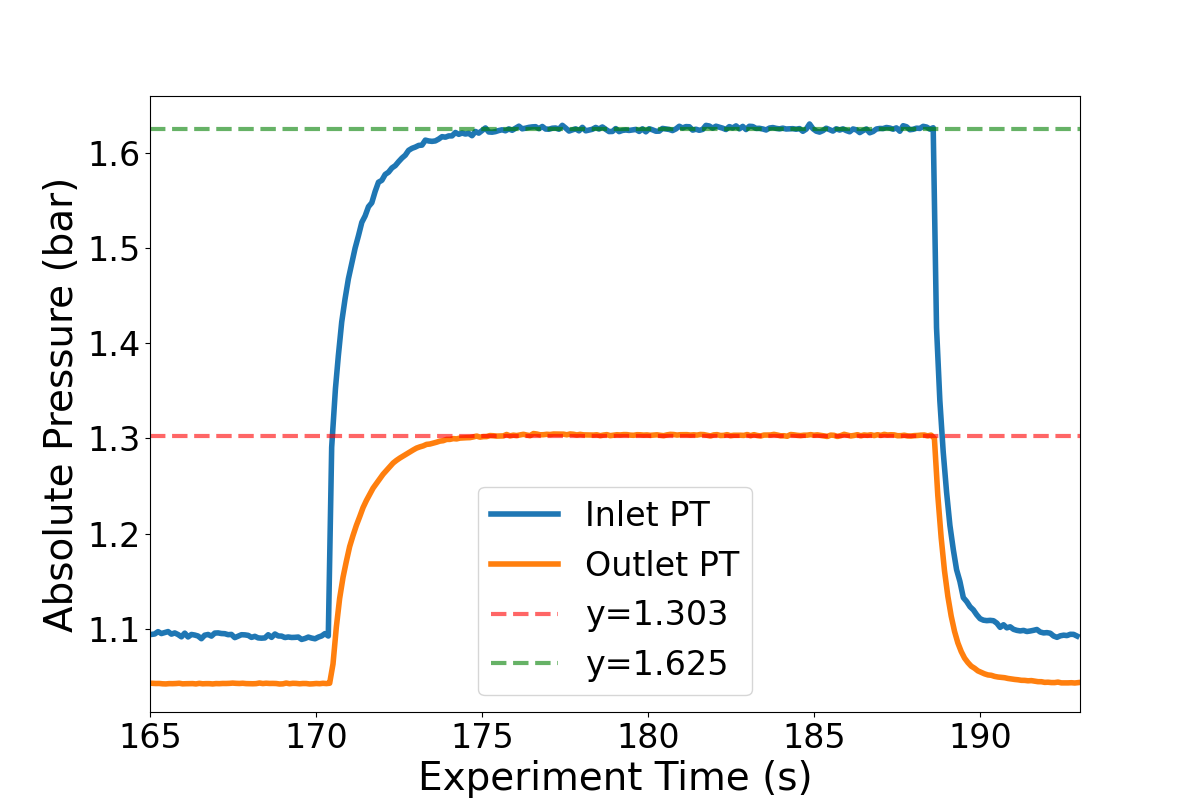
\includegraphics[width=\textwidth]{../report_assets/4_bar_static.png}
        \caption{Static pressure from 5 bar.}\label{fig:static-pressure-drop-4bar}
    \end{minipage}
    \hfill
    \begin{minipage}{0.45\textwidth}
        \centering
        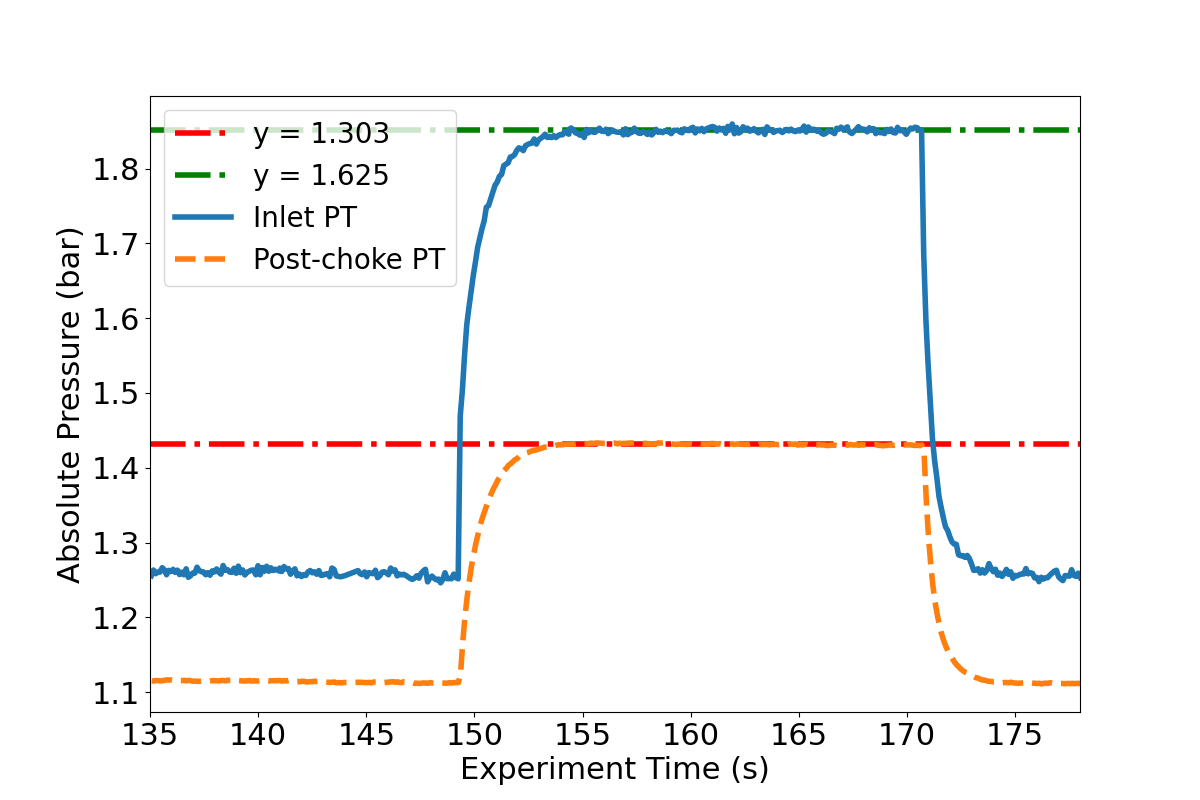
\includegraphics[width=\textwidth]{../report_assets/5_bar_static.png}
        \caption{Static pressure from 6 bar.}\label{fig:static-pressure-drop-5bar}
    \end{minipage}


\end{figure}
If the compressed air line was truely supplying a stagnation pressure of 4 bar, through isentropic flow relations the data implies that the mach number of the flow is 1.3 which is unlikely.

As seen in \autoref{fig:static-pressure-drop-3bar_full}, the regulator was able to control the static pressure to 4 bar when the system was closed. When the system opens, one could expect that the regulator would maintain this 4 bar static pressure and only static pressure losses in the system and acceleration of the flow beyond the regulator would reduce it somewhat. However, by the time the flow reached the pressure transducer before the tank, the static pressure had dropped to 1.4 bar. 

Assuming the flow was mach 1 through the nylon pipe, this would imply a stagnation pressure of roughly 2 bar not the 4 bar initially desired.

\subsection{Further Investigation}
In an attempt to diagnose this behaviour, a follow up test was conducted to check whether this was due to an incorrect system set up or was a product of the compressed air line.
To further investigate this behaviour, the pressure regulator connected to the compressed air line was set to max (roughly 7bar) and a second regulator was introduced closer to the system. If the problem was large static pressure losses from the long nylon tube connecting the inlet of the experiment to the pressure source, a larger pressure during operation would have been observed. Additionally, if the pressure regulator was faulty or some other weird behaviour was occuring upstream of the setup, this could have indicated that.
As seen in figure the performance was much worse giving even lower static pressure readings. 
\begin{figure}[htbp]
    \centering

    \begin{minipage}{0.45\textwidth}
        \centering
        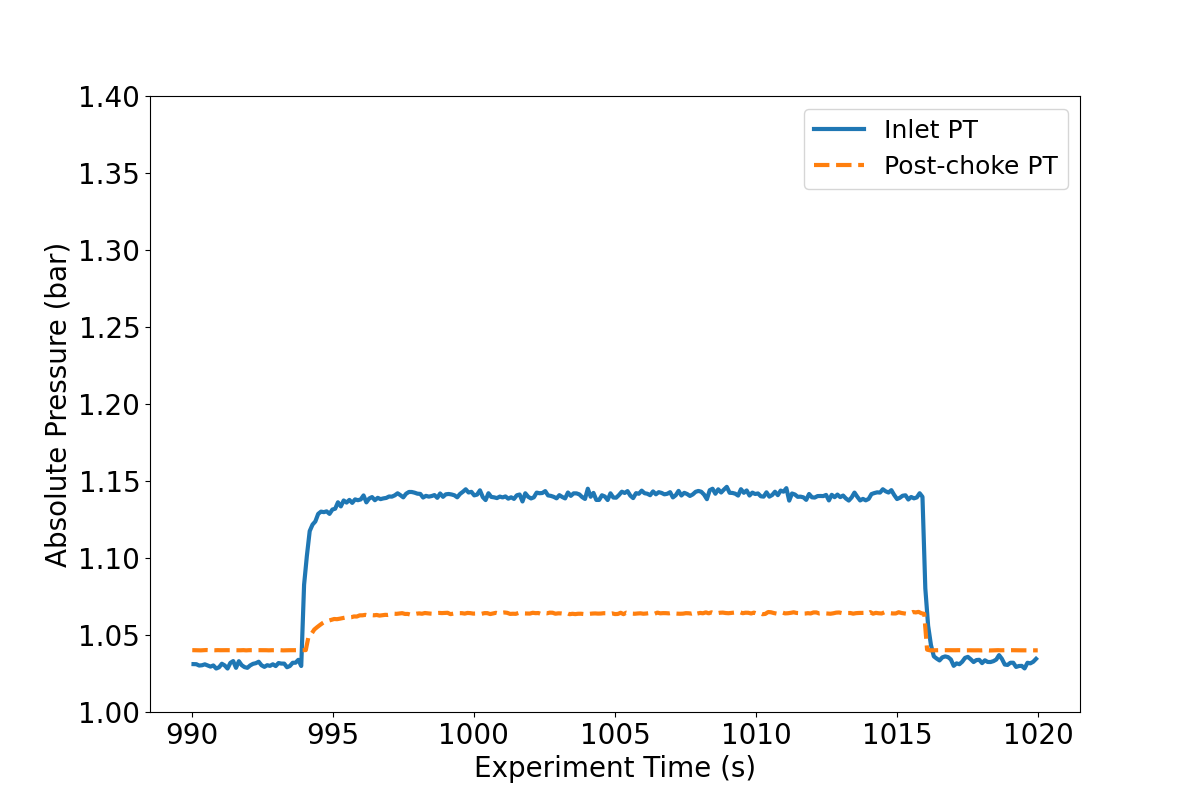
\includegraphics[width=\textwidth]{../report_assets/3_bar_static_new_reg.png}
        \caption{New regulator.}\label{fig:static-pressure-drop-new-reg}
    \end{minipage}
    \hfill
    \begin{minipage}{0.45\textwidth}
        \centering
        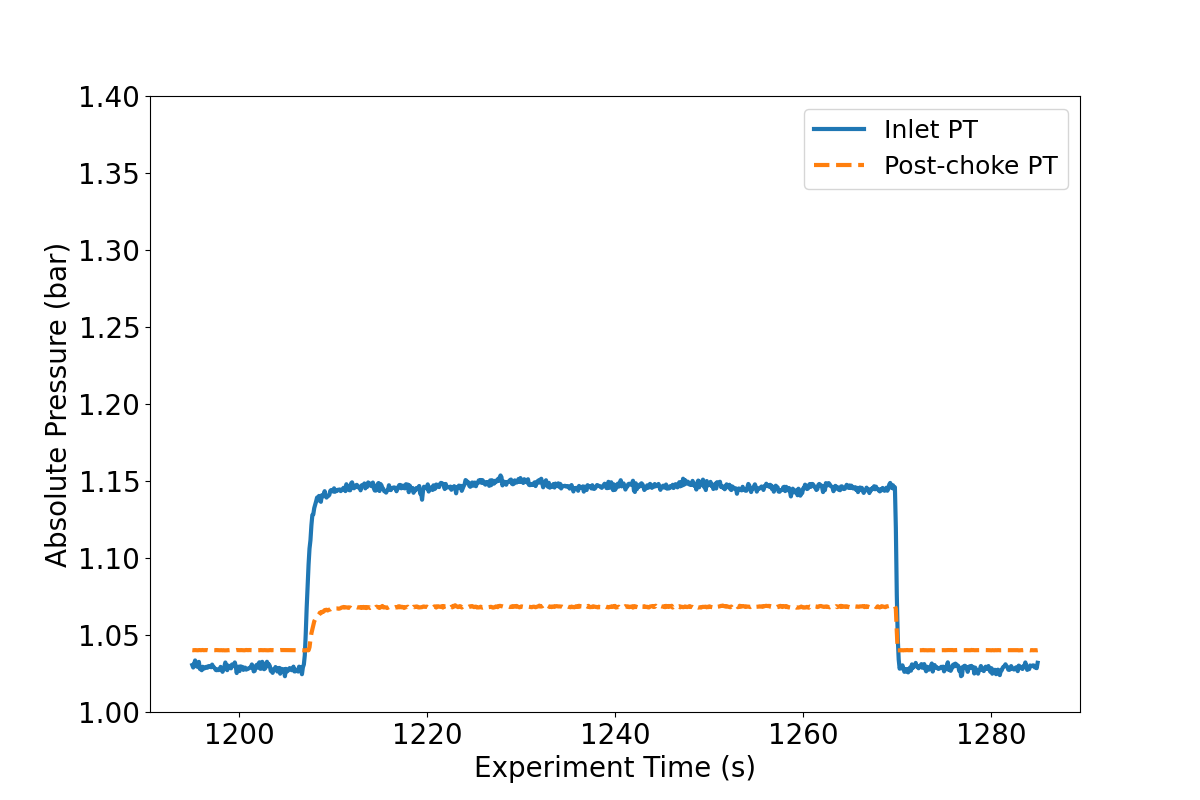
\includegraphics[width=\textwidth]{../report_assets/3_bar_static_no_solenoid.png}
        \caption{New regulator + no solenoid.}\label{fig:static-pressure-drop-no-solenoid}
    \end{minipage}

\end{figure}
As a final attempt, the solenoid valve was removed from the set up to verify that this wasnt choking the flow or somehow drastically decreasing static pressure somehow. Again, seen in fig 6, this performed similarly to the setup containing the regulator so wasn't the cause of the behaviour and the system diagram was reverted to \autoref{fig:systems-diagram}.
\subsection{Simulation}
A 2D Axisymmetric analysis of the empty tank was conducted using fluent. This seemed to support the idea that only 1bar of stagnation pressure was being supplied to the system, not the desired 3bar as setting the pressure inlet to 1bar gave comparable static pressure readings as seen in the tests.
\begin{figure}[htbp]
    \centering

    \begin{minipage}{0.45\textwidth}
        \centering
        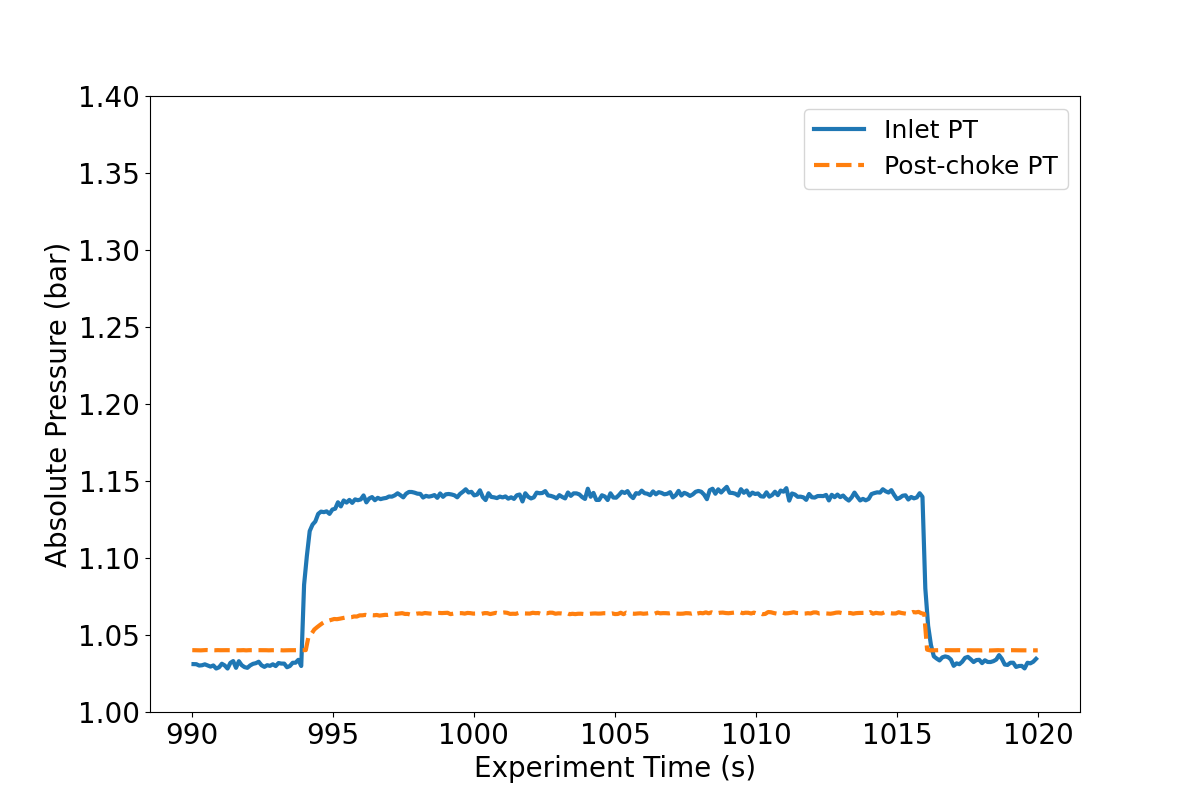
\includegraphics[width=\textwidth]{../report_assets/3_bar_static_new_reg.png}
        \caption{New regulator.}\label{fig:static-pressure-drop-fluent}
    \end{minipage}
    \hfill
    \begin{minipage}{0.45\textwidth}
        \centering
        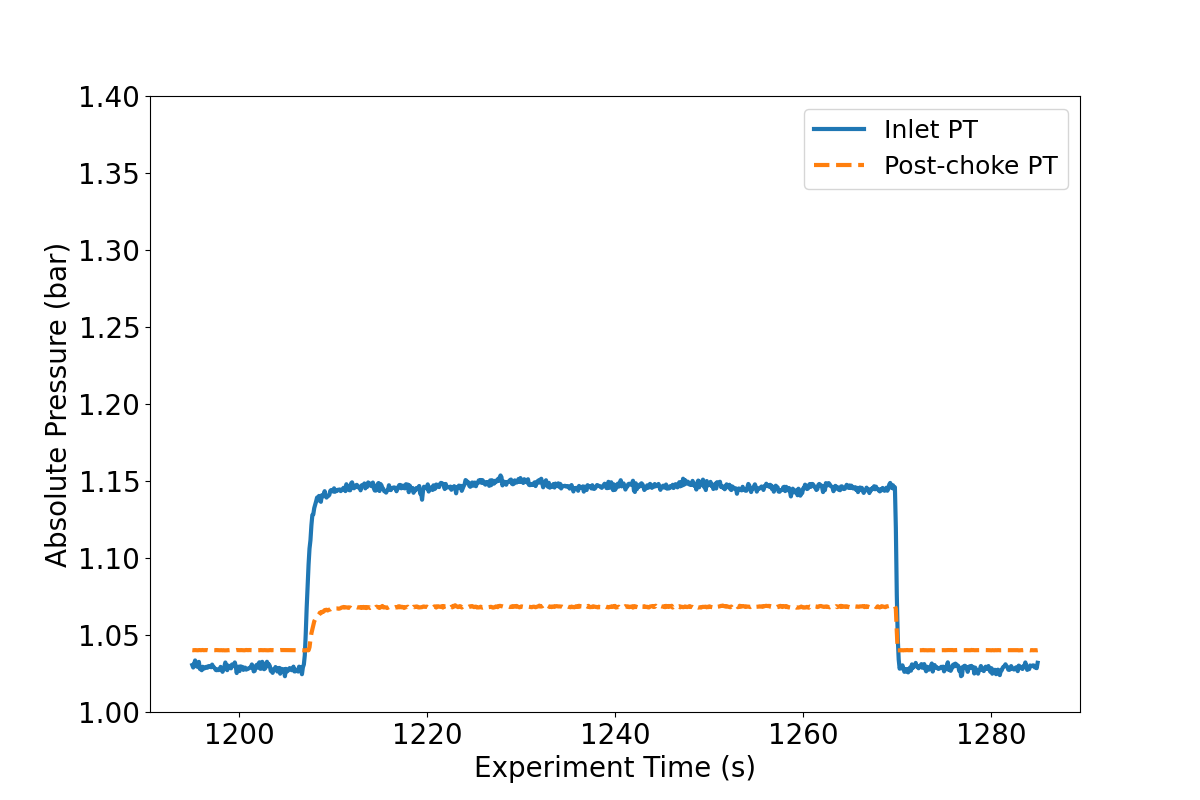
\includegraphics[width=\textwidth]{../report_assets/3_bar_static_no_solenoid.png}
        \caption{New regulator + no solenoid.}\label{fig:static-pressure-drop-report}
    \end{minipage}

\end{figure}


\section{first test}
yappa yappa
\begin{figure}[htbp]
    \centering

    \begin{minipage}{0.45\textwidth}
        \centering
        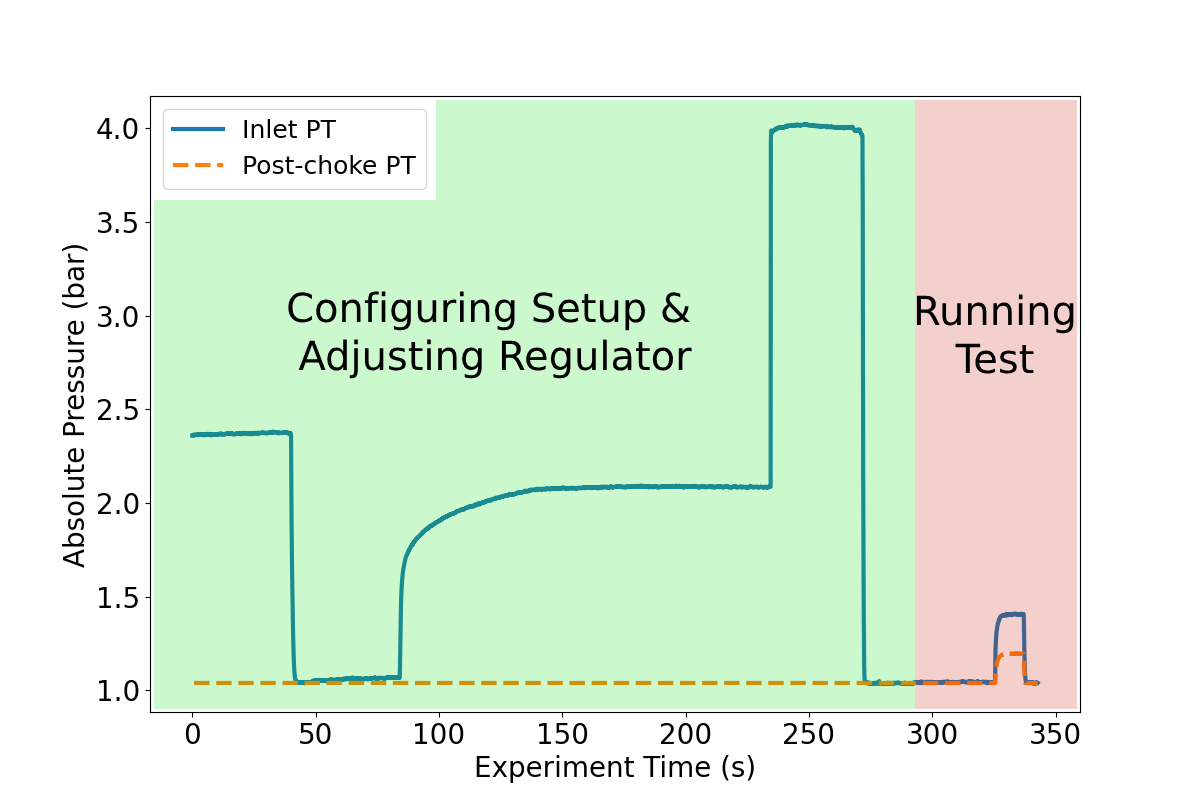
\includegraphics[width=\textwidth]{../report_assets/3_bar_static_full.png}
        \caption{pressure readings full.}\label{fig:static-pres-drop-3bar_full}
    \end{minipage}
    \hfill
    \begin{minipage}{0.45\textwidth}
        \centering
        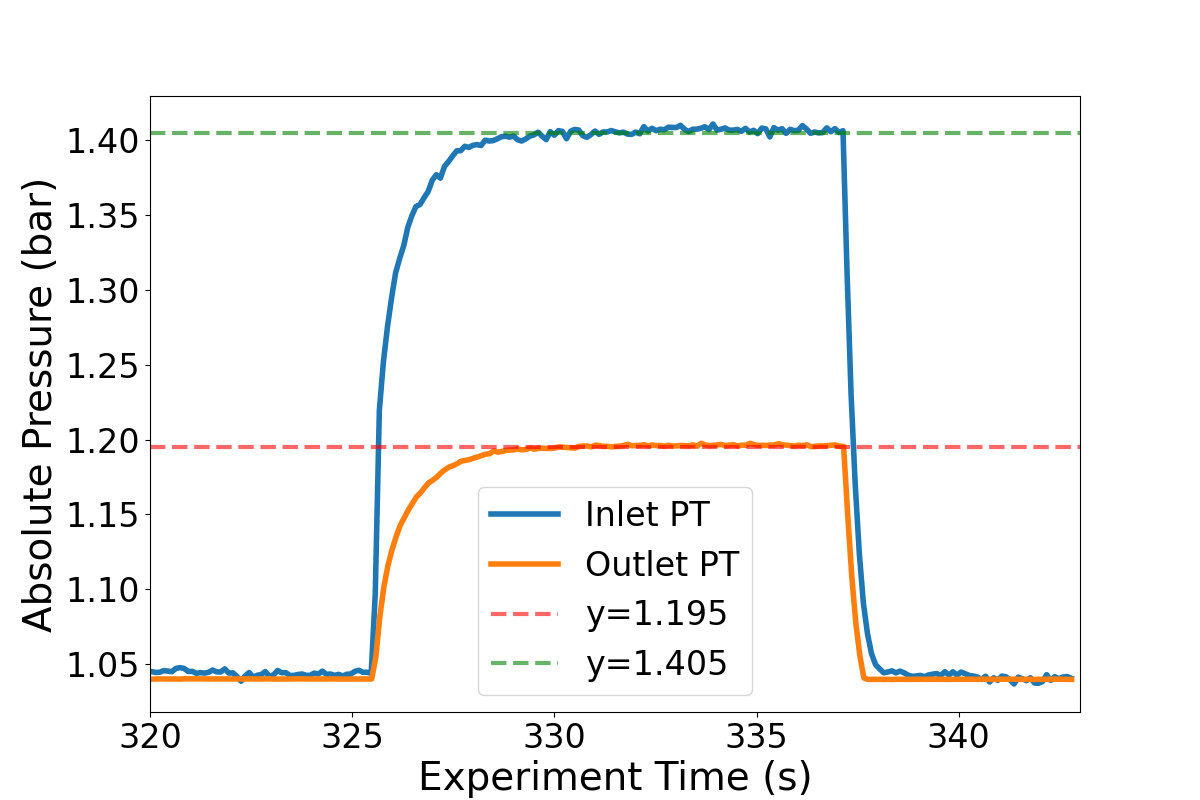
\includegraphics[width=\textwidth]{../report_assets/3_bar_static.png}
        \caption{pressure readings of 3bar gauge.}\label{fig:static-pressurop-3bar}
    \end{minipage}

\end{figure}
highlighted the issue of the piston locking up,
force required to compact the sand to the outlet
sand only at the top moved
no fluidisation behaviours observed, maybe higher pressures required after all
chokepoint blocked sand and prevented flow into cyclone seperator
\section{Piston velocity - mass flow rate relation}
didnt really work. idk why but it should have
\section{Piston design}
due to granular material being bigger than typical, often gets stucka round the piston and causes it to lock up

redesign
modelling the piston as a circle and the sand as a fluid. 
P = rho * h * g
P = 1529 * (74mm - y) * 9.81~= 15000* (74mm - y)
\begin{equation}
    \int_{-0.037}^{0.037}\!\int_{0}^{0.037+\sqrt{0.037^2 - x^2}}15000\,(0.074 - y)\,\mathrm{d}y\,\mathrm{d}x
    \;-\;
    \int_{-0.037}^{0.037}\!\int_{0}^{0.037-\sqrt{0.037^2 - x^2}}15000\,(0.074 - y)\,\mathrm{d}y\,\mathrm{d}x.
\end{equation}

% \begin{equation}
%     15000\int_{-0.037}^{0.037}\Bigl(0.037^2 + \frac{x^2}{2} + 0.037\sqrt{0.037^2 - x^2}\Bigr)\,\mathrm{d}x = 0.302369.
% \end{equation}
% \begin{equation}
%     15000\int_{-0.037}^{0.037}\Bigl(0.037^2 + \frac{x^2}{2} - 0.037\sqrt{0.037^2 - x^2}\Bigr)\,\mathrm{d}x = 0.302369.
% \end{equation}
\begin{equation}
    15000\int_{-0.037}^{0.037}\Bigl(0.037^2 + \tfrac{x^2}{2} + 0.037\sqrt{0.037^2 - x^2}\Bigr)\,\mathrm{d}x
    \;-\;
    15000\int_{-0.037}^{0.037}\Bigl(0.037^2 + \tfrac{x^2}{2} - 0.037\sqrt{0.037^2 - x^2}\Bigr)\,\mathrm{d}x
\end{equation}
\begin{equation}
    15000\int_{-0.037}^{0.037}\Bigl(0.074\sqrt{0.037^2 - x^2}\Bigr)\,\mathrm{d}x = 2.38697N
\end{equation}

555.001308106 Pa average pressure differential across the two piston faces to get this force required to compact the sand

deltaP for fluidising bed is $h*(rho_s - rho_a)*9.81$ which is 0.2 1527 10 = 300pa


sand drops static pressure only. Therefore probably need to make the piston drop about half a bar of static pressure aswell
this is easily testable in the setup

need to think about friction when testing for a certain dp across the faces

need to think about the sand when designing for the geometry so it doesnt get stucka

might run into the inherent cocking issue since pressure from sand is concentrated at the bottom

static pressure losses from the tank and set up alone

3 bar (gauge) stagnation goes to 1.405bar static and 1.195bar static = loss of 0.210bar static
4 bar (gauge) stagnation goes to 1.625bar static and 1.303bar static = loss of 0.322bar static
5 bar (gauge) stagnation goes to 1.852bar static and 1.432bar static = loss of 0.420bar static

static pressure losses from the tank + piston

3 bar (gauge) stagnation goes to 1.425bar static and 1.209bar static = loss of 0.216bar static
4 bar (gauge) stagnation goes to 1.628bar static and 1.304bar static = loss of 0.324bar static
5 bar (gauge) stagnation goes to 1.831bar static and 1.431bar static = loss of 0.400bar static

static pressure losses from the tank + new piston

3 bar (gauge) stagnation goes to 1.423bar static and 1.205bar static = loss of 0.218bar static
4 bar (gauge) stagnation goes to 1.645bar static and 1.311bar static = loss of 0.334bar static
5 bar (gauge) stagnation goes to 1.850bar static and 1.450bar static = loss of 0.400bar static

